\chapter*{Lecture 1}

\section*{Context of the course}


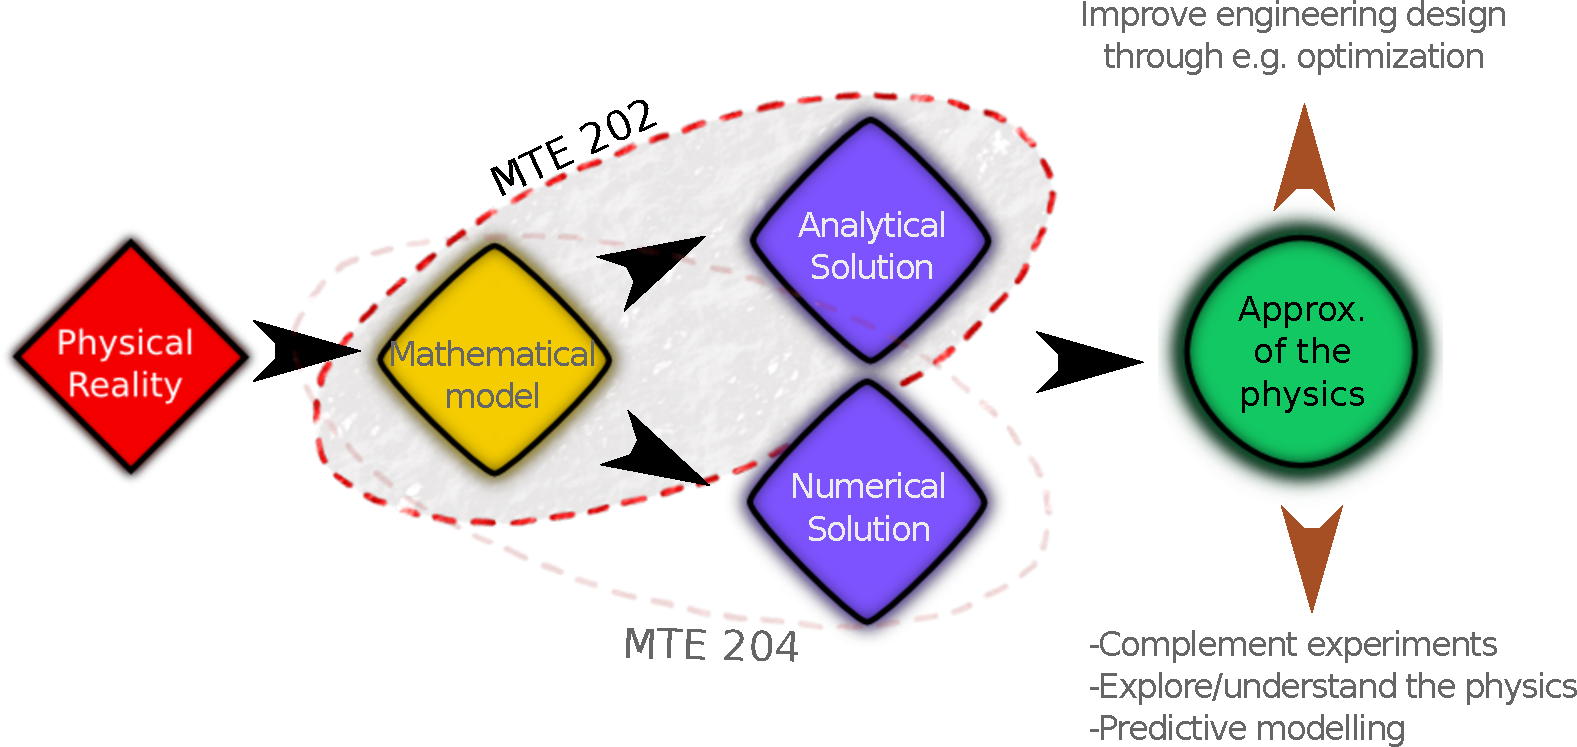
\includegraphics[width=0.9\textwidth]{figs/ConceptMap.pdf} 




\section{What is a differential equation?}

\begin{itemize}
\item In the language of mathematics, changing entities are called \textbf{variables} and the rate of change of one variable with respect to another a \textbf{derivative}.
\item Equations which express a relationship between the variables and their derivatives are called differential equations
\item We are NOT interested in knowing how the variables and derivatives are related but only how the variables themselves are related.
\end{itemize}

For example, knowing the position of a particle with regards to its rate of change with respect to time is not particularly instructive. We seek to determine the position of the particle with respect to any time $t$!



\section{Algebraic vs differential equations}
We are typically comfortable with \emph{algebraic equations} or  \emph{polynomial equations}  of the form:
\begin{equation}
x^2+3x-4=0
\end{equation}
In the above example, we seek to find the \emph{value} or \emph{set of values} of $x$ which satisfy the algebraic relation. In this example, we have the values of $x=-4$ and $x=1$ which satisfy the relation.
A differential equation may take a very similar form:
\begin{equation}
y''+3y'-4=0
\end{equation}
where $y$ is a function of an independent variable, say $t$. But in this case, we try to find a \emph{function} or \emph{set of functions} that satisfy the above differential equation. In this course, you will learn how to classify differential equations and determine the correct solution strategy to solve them analytically.

Now, let us consider a very simple differential equation:
\begin{equation}
\frac{d y}{dx}=y
\end{equation}
Intuitively, what does this represent? If we were to write out this equation in words, we would say: "the slope of the function $y$ must equal to the position $y$". We can represent this graphically...

\begin{testv}{Story of the radioactive decay}{}
%\begin{exmp}{Story of the radioactive decay} %Tenenbaum book
Carbon dating: ODE example
\begin{itemize}
\item Teenagers walking through the forest in September 1940 near the town of Lascaux, France
\item They lost a dog in cave; the teenagers went to retrieve the dog
\item On the wall of the ancient cave, they found paintings of horses, cattle, beasts etc
\item Also found the remains of a charcoal fire in the cave
\end{itemize}
The problem was to determine when these paintings were made?\\
The key to this problem lies in understanding the physics/chemistry of the problem
\begin{itemize}
\item Charcoal is burnt wood
\item Changes take place in all dead organic matter
\item All living organisms contain two isotopes of carbon $C^{12}$ (stable) and $C^{14}$ (radioactive, 6 protons/8 neutrons)
\item In living organisms the ratio of $C^{12}$ to $C^{14}$ remains constant
\item When an organism dies, the radioactive $C^{14}$ is lost and not replaced
\end{itemize}
If $t$ represents the time elapsed since the tree died and let $x$ be the amount of $C^{14}$ present in the dead tree at any time. The instantaneous rate at which $C^{14}$ decomposes is then:
\begin{equation}
\frac{dx}{dt}
\end{equation}
We make a further assumption that $C^{14}$ varies to the first power of $x$ (in other words, the more $C^{14}$ present, the faster the decomposition)
\begin{equation}
\frac{dx}{dt}=-kx
\end{equation}
where $k$ is a proportionality constant (which is negative since $x$ is decreasing).
If we know the amount of $x$ at any given time, we can determine a date at which the organism stopped living. 
\end{testv}


\section*{Common Terminology}
\subsection*{Dependant vs Independent variable}
If an equation involves the derivative of one variable with respect to another, then the former is called a \textbf{dependent variable} and the latter an \textbf{independent variable}.

\subsection*{Function}
If to each value of an independent variable there corresponds one and only one value of the dependent variable, we say that the dependent variable is a \textbf{function} of the independent variable. We can write a function in the form $f(x)$ where $x$ is the independent variable. It should be noted that $f(x)$ can also be a constant!
\begin{center}
\noindent\rule{4cm}{0.4pt}
\end{center}

\begin{exmp}{}
The temperature $T$ of a body is recorded over a 24 h period (see fig \ref{Fct}). The horizontal axis represents  time in hours, the vertical axis the temperature in Celsius.
\begin{figure}
\centering
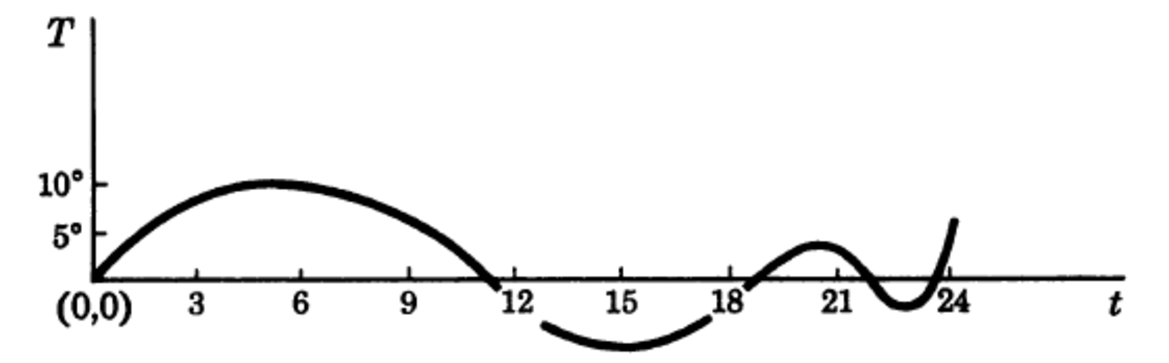
\includegraphics[width=0.5\textwidth]{figs/function.pdf} 
\caption{Function example\label{Fct}}
\end{figure}
For each value of time $t$, there is a unique value of temperature $T$. Hence the graph defines $T$ as a function of $t$. (we don't even need an explicit relation between $t$ and $T$ to state that there is a functional dependence between them). We can write $T=f(t)$. $\bLozenge$
\end{exmp}


\begin{exmp}{Falling object:}{}
Let's consider a falling object. Formulate a differential equation that describe its motion.\\
\textbf{Solution:}
We will denote time using $t$. The velocity of the object, $v$, will presumably change with $t$. So $v$ will be a function of $t$: $v(t)$. In this case, $t$ is the independent and $v$ the dependent variable.\\
The physical law governing the motion of the falling object is \textbf{Newton's second law}:
\begin{equation}
F=ma
\end{equation}
where $m$ is the mass of the object, $a$ its acceleration, and $F$ the net force of the object. As we know, acceleration, $a$, is related to the change of $v$ with respect to $t$: $a=dv/dt$.\\
\begin{equation}
F=m\frac{dv}{dt}
\end{equation}
Let's now consider the forces acting on the object. 
\begin{itemize}
\item Gravity: exerts a force equal to the weight of the object: $mg$, where $g$ is the gravitational acceleration equal to 9.8 $m/s^2$.
\item Drag: without going into detailed fluid mechanics, we assume that drag is proportional to the velocity: $\gamma v$, where $\gamma$ is the drag coefficient.
\end{itemize}
\begin{equation}
F=mg-\gamma v
\end{equation}
The resulting ODE becomes:
\begin{equation}
m\frac{dv}{dt}=mg-\gamma v
\end{equation}
To solve this ODE, we need to find function $v(t)$ which satisfies this equation. $\bLozenge$
\end{exmp}
\updateinfo[September 10, 2018]

